\documentclass{sig-alternate}
\usepackage{amsmath,amsfonts}
\usepackage{booktabs}
\usepackage{multirow}

\begin{document}

\title{Learning to Assess the Cognitive Capacity of Human Partners}

\numberofauthors{3} 

\author{
%
\alignauthor
Anonymous\\
% Matthew Atkins\\
%        \affaddr{Oklahoma State University}\\
%        \affaddr{Robotics Cognition Laboratory}\\
%        \affaddr{Stillwater, Oklahoma 74078}\\
%        \email{matthew.atkins@okstate.edu}
% % 2nd. author
% \alignauthor
% S. M. Al Mahi\\
%        \affaddr{Oklahoma State University}\\
%        \affaddr{Robotics Cognition Laboratory}\\
%        \affaddr{Stillwater, Oklahoma 74078}\\
%        \email{smahi@okstate.edu}
% % 3rd. author
% \alignauthor Christopher Crick\\
%        \affaddr{Oklahoma State University}\\
%        \affaddr{Robotics Cognition Laboratory}\\
%        \affaddr{Stillwater, Oklahoma 74078}\\
%        \email{chriscrick@cs.okstate.edu}
}

\maketitle
\begin{abstract} 
We demonstrate that a robot is capable of learning to recognize the
behavioral indicators that a complex, rapidly-evolving task has exceeded
the cognitive capacity of a human partner and make an informed decision
based upon this assessment.
\end{abstract}

%\category{I.2.9}{Robotics}{Human Assistance}{Multiple Robots}

%\terms{Cognitive Limitation, Trust, Mobile Robot}

\keywords{User modeling and awareness, teamwork and group dynamics,
  robot behavior design, quantitative field study, learning about the
  environment}

\section{Introduction}
One of the most challenging obstacles facing human-robot teams is the
inherent communication barrier between the two. Human operators, at
least once they have received training, have some notion concerning
the capacities of their mechanized partners, but the ability of robots
to assess the limitations of humans has not received adequate
attention.

The robot is trained to associate human directions with task quality for a well-understood task, in this case, the
navigation of a maze. The robot may then apply this learned model to a
different problem while still being able to evaluate a human operator's
cognitive load. Even without the ability to understand the end goal of this
new task. Human-robot interactions can be evaluated using fundamental metrics
\cite{olsen2003metrics} like task effectiveness (TE), neglect tolerance (NT), free time (FT), fan out (FO).
Physiological metrics as objective evaluation along with subjective evaluation for cognitive load estimate\cite{Brookings1996361}.

\section{Problem statement} Take $H=[h_1,h_2,\cdots,h_m]$ to be a vector of ecologically
valid measurements of human behavior relevant to the problem space.  Assume a task for which a robot participant can
independently calculate $s$ which is a function of a vector of measurable environmental features
$E=[e_1,e_2,\cdots,e_n]$.  Thus, $s = f(E)$, where $f$ is a task-specific function known to the robot.  Using $f$ and
calculating $s$, a robot can build its own supervised training set for a learning task, where the human input $H$ is
associated with $s$ through a learned function $g$.  Thus, the robot learns to associate the human behavioral metrics
$H$ with task success $s$ within a known task, so the output of $g$ is a learned \emph{estimate} of the true success
($\hat{s}=g(H)$).  Now, assign the robot a task which requires human input for success, i.e., the robot has no access to
an analogue to $f$ or $s$ in this new task.  However, it can still measure the components of $H$, and it has access to
its learned model $g$.  We show that computing $\hat{s}=g(H)$ in this new environment allows the robot to estimate not
the task success, but the cognitive load on its human partner and an estimate of the quality of the human's direction.

\section{Experimental design} 
Our experiments consisted two games, namely, the Maze and the Coin. Effectively
navigating a Maze game has been demonstrated in literature \cite{crick2011human}. In the Mage game, the robot collected
the data needed to build a model $g$ for evaluating the trustworthiness of user input $H$. In the subsequent Coin Game,
the robot is placed in a different scenario, one in which it had no access to success measures or even rules; beyond the
fact that it was moving in a similar environment to the Maze Game. Even so, with no independent means of measuring task
success, it can still calculate $\hat{s}=g(H)$, and can therefore evaluate the quality of instruction, and hence the
cognitive capacity, of its human partner. Communication between operators and robots was achieved using the Robot Operating System (ROS).

In the Maze Game,  vector of environmental measurements $E = [e_0, e_1, e_2]$.In this particular context,$e_0$ is the
\emph{disparity} term, the distance between the navigation directions provided by a human and the route that the robot
would have planned for itself,$e_1$ is the \emph{collision} term, which penalizes collisions with walls, and $e_2$ is
the \emph{time delay} term, the amount of time taken for the human to guide the robot through the maze, compared with
the robot's estimate of the time it would have taken under its own power. The computation of $s = f(E)$ is a function
for measuring success of the human directions , is a normalized summation of all metric in $E$.

By computing this value $s$, the robot can label its own data in order to train a supervised learning algorithm which
will relate the success of a human-directed task with a set of measured behaviors $H = [h_0, h_1, h_2]$. For this particular experiment,$h_0$ is the \emph{decision interval}
term, which measures the time elapsed between the robot reaching a navigation goal and the human providing a new one,
$h_1$ is the \emph{error correction} term, which measures the tendency of a human operator to provide a navigation goal
and then subsequently provide another before the task is complete, and , $h_2$ is the \emph{franticness} term, which
characterizes erratic behavior for the control inputs.

\section{Results} In general, the robot correctly predicts the cognitive load that its operator was under in every
scenario Fig~\ref{fig:coder_eval_1_2}. From our experiments we
have found that the cognitive load estimate from the robots using our model correlates with the coder evaluated stress
level by a factor $\rho=.205$ and $\rho=.25$ for coin game played with one and two robots respectively. Our experiment
also captures that posture and breathing rate of human operator as objective metric for estimating cognitive stress
level.We could not find any interesting pattern in other physiological objective metrics i.e. heart rate, ECG amplitude
using our model and experimental setup.The benefits of this can be seen in Fig~\ref{fig:BoxWiskersTimeComp}.  It is critical for interpreting the information in
Fig. \ref{fig:coder_eval_1_2} or \ref{fig:pred_phy} to note that while the robot's cognitive load evaluation and the
scoring technique for quantifying self-reported user stress both produce a result between zero and one \textit{their
magnitudes are not directly comparable}.Whenever cognitive stress occurs or changes, the robot is able to recognize this
increase for most cases in the tested scenarios, and the robot's evaluation agrees with self-reported user stress.

\begin{figure}  
\centering
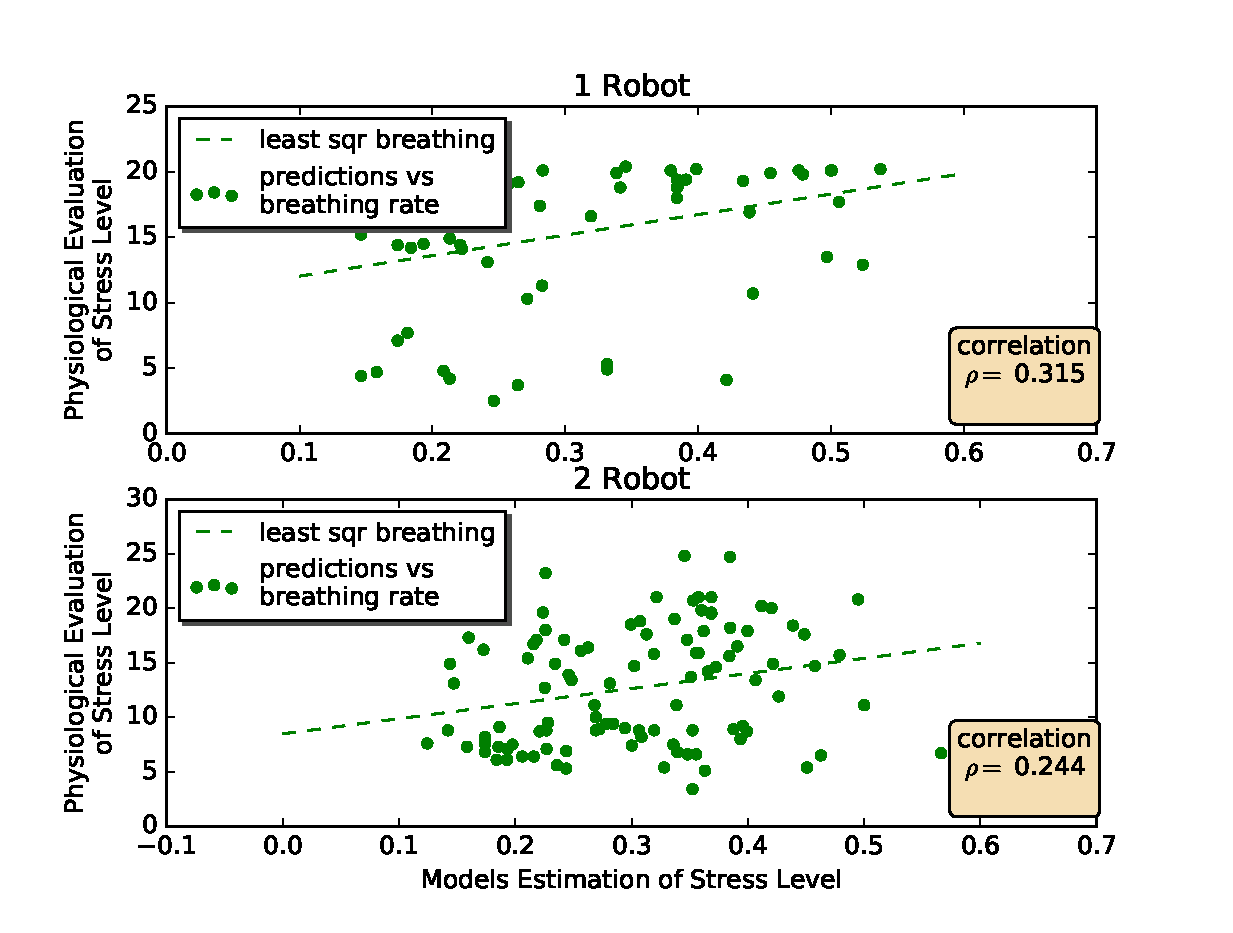
\includegraphics[width=.5\textwidth]{prediction_vs_b_p_2.eps}
\caption{Models predicted stress level vs Physiological metrics in coin game experiment.}
\label{fig:pred_phy}
\end{figure}

Most important contribution of our model can has been demonstrated from the perspective of task success. The task
success of the coin game is measured in term of number of coins collected within given time. Task success score has been quantified as the duration of the game penalized by a constant score in case of a failure. Tab.\ref{tab:task_success}.
It shows that autonomous assistance improves overall task success score. In the context of this paper, it also supports the
original hypothesis: robots are able to reliably assess the cognitive strain their human partners are under, even in
contexts where the actual tasks they are being asked to perform are opaque to the robot.

\begin{figure}
\centering
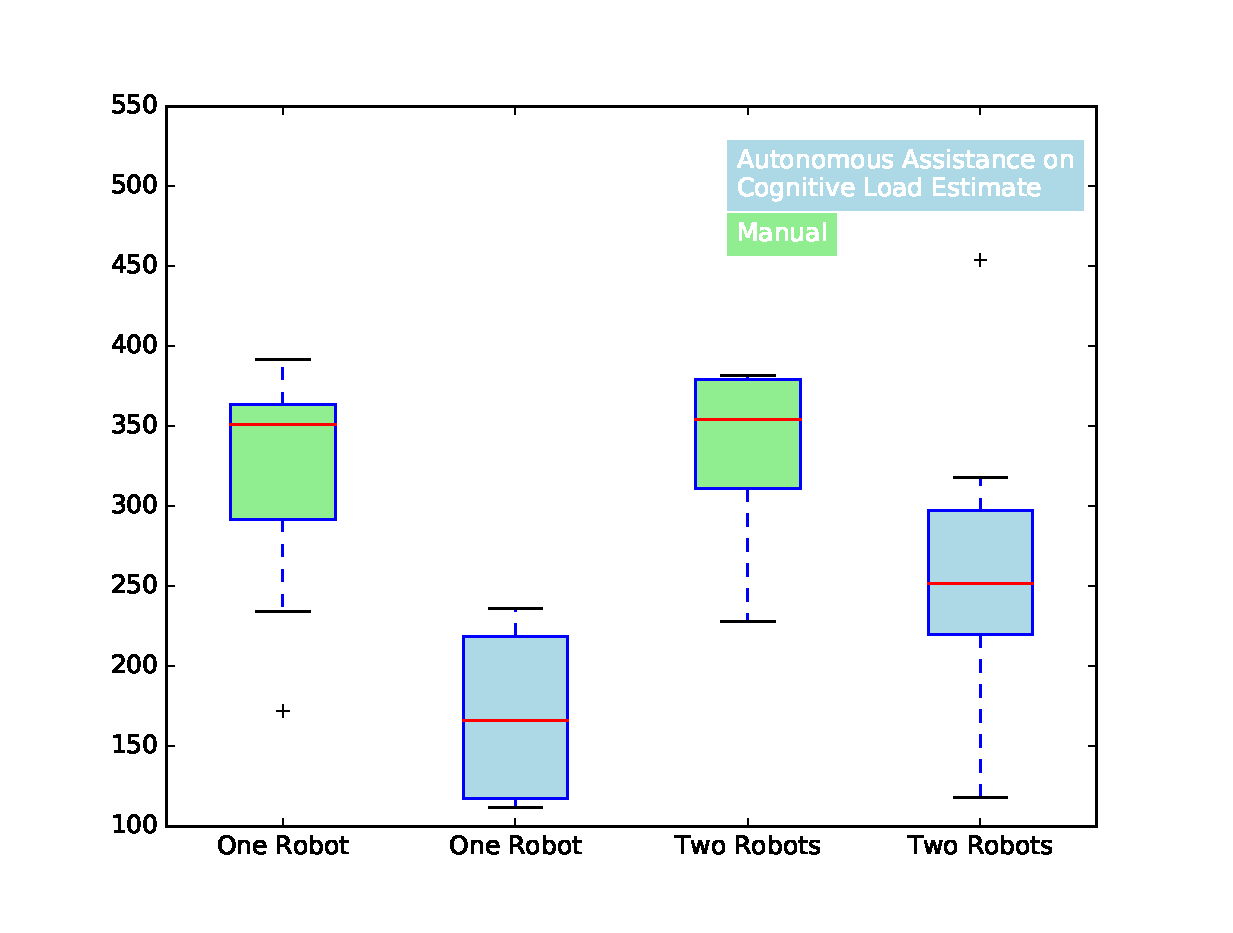
\includegraphics[width=.5\textwidth]{BoxWiskerTimesCompMaualVsAuto2.eps}
\caption{Comparison of task task success for task involving one and two robots operating in both manual and autonomous modes. Task success has been quantified as task completion time with additional penalty for failure to complete the task (loosing the Coin game).}
\label{fig:BoxWiskersTimeComp}
\end{figure}

\begin{table}[] \centering \caption{Task success comparisons between autonomous assistance mood and manual mood.
Autonomous assistance was activated on detection of high stress level predicted by our model.} \label{tab:task_success}
\begin{tabular}{@{}|c|c|c|c|c|@{}} \toprule Game Mode & \multicolumn{2}{c|}{Manual} &
\multicolumn{2}{c|}{\begin{tabular}[c]{@{}c@{}}Autonomous \\ Assistance on high\\ Stress level\end{tabular}} \\ \midrule
\begin{tabular}[c]{@{}c@{}}Number of\\ Robots\\ Participated\end{tabular} & one     & two  & one  & two  \\ \midrule
\begin{tabular}[c]{@{}c@{}}Number of Failure/\\ Total Number\\ of Game Played\end{tabular} & 3/7 & 3/7 & 0/10 & 1/10 \\
\midrule \begin{tabular}[c]{@{}c@{}}Task Success Score\\ per game\end{tabular}                & 318  & 355  & 170  &
258.2   \\ \bottomrule \end{tabular} \end{table}

\begin{figure}
\centering
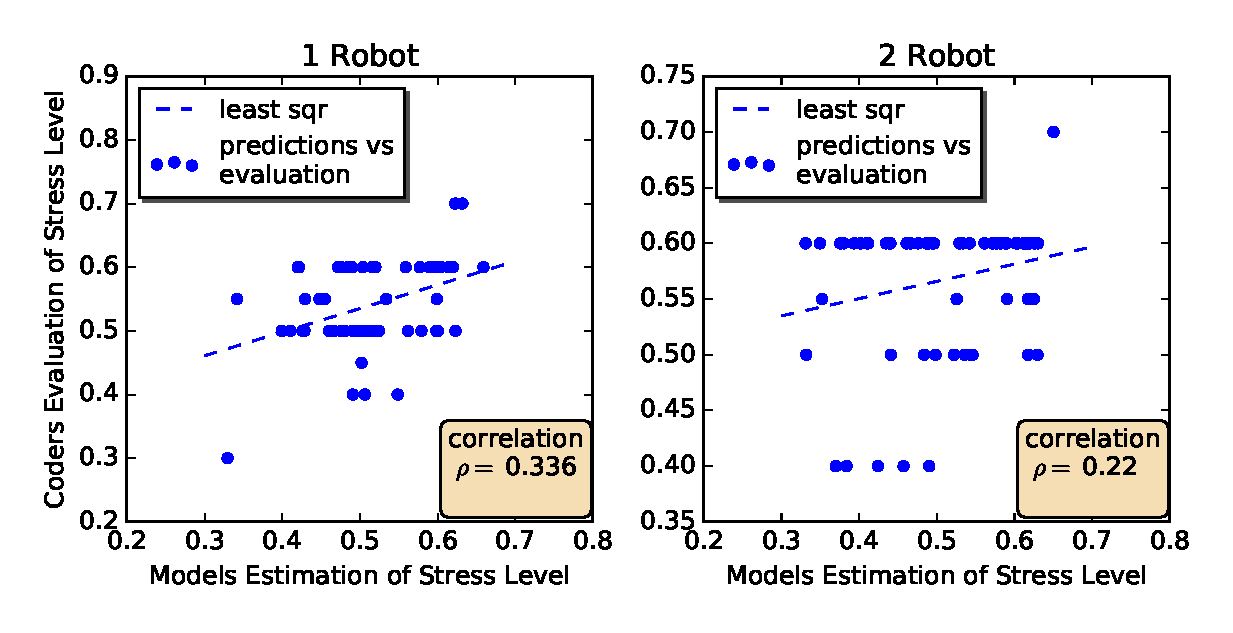
\includegraphics[width=.5\textwidth]{coder_eval_1_2.eps}
\caption{Cognitive load of human operators in Coin Game experiments with differing numbers of robots and steadily increasing task complexity. The robots' predictions fairly correlates with the coder evaluation of cognitive load estimate.}
\label{fig:coder_eval_1_2}
\end{figure}


\section{Conclusions}

Every day humans interact with more and more technologies that require us to decide whether or not to trust them; robots
should be making similar determinations about us.In the future, we plan to extend this research into complex
heterogeneous teams of humans and robots performing real-world tasks.

\section{Acknowledgments}

%We would like to thank Robotic Cognition Laboratory of Computer Science Department of Oklahoma State University for facilitating this project. We would also like to thank all the people who participated in the project as human operator voluntarily.

\bibliographystyle{abbrv}
%\bibliographystyle{acmlarge}
\bibliography{sigproc-2}

\end{document}
